\section{Escritorio KDE}
\subsection{Presentaciones}
\frame
{
  \frametitle{La ``K'' y Konqui}
  \begin{center}
    \includegraphics[height=3cm,width=3cm]{./imgs/logo.jpg}
    \hspace{2cm}
    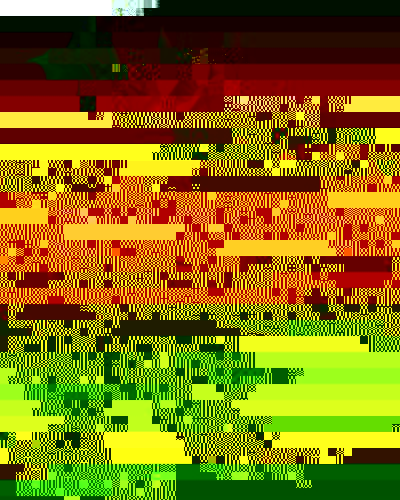
\includegraphics[height=4cm,width=3cm]{./imgs/konqui.jpg}
  \end{center}
}
\frame{
	\frametitle{Tux}
	\begin{center}
    \includegraphics[height=6cm]{./imgs/Penguin.png}
	\end{center}	
}

\subsection{Entrando al sistema}
\frame
{
  \frametitle{KDM}
  \begin{center}
    
\includegraphics[height=5cm]{./imgs/kdm}
  \end{center}

}
\subsection{Aspecto Bardinux}
\frame
{
	\begin{center}
		
\includegraphics[width=8cm]{./imgs/kde_bardinux.jpg}
	\end{center}
}
\subsection{El kicker (la barrita de abajo)}
\frame
{
	\frametitle{El kicker}
	\begin{center}
		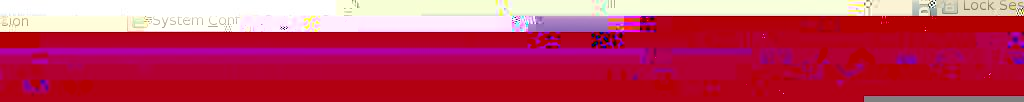
\includegraphics[height=1cm,width=10cm]{./imgs/kicker.jpg}
	\end{center}
	\begin{itemize}
		\item{El menú K}
		\item{El paginador de escritorio}
		\item{La bandeja del sistema}
	\end{itemize}
}
\frame
{
	\frametitle{Algunos Applets Más}
	\begin{itemize}
		\item<1->{Menú K}
		\item<2->{Paginador de Escritorios}
		\item<3->{Barra de tareas}
		\item<4->{Bandeja del sistema}
		\item<5->{Paginador y previsualizador del escritorio}
		\item<6->{Papelera}
		\item<7->{Klipper}
	\end{itemize}
}
\subsection{Configurar KDE}
\frame
{
	\frametitle{KControl}
	\begin{center}
		
\includegraphics[height=6cm]{./imgs/kcontrol.jpg}
	\end{center}
}
\frame
{
	\frametitle{Preferencias del sistema}
	\begin{center}
		\includegraphics[height=6cm]{./imgs/pref_sistema.jpg}
	\end{center}
}
%\frame
%{
%	\large{La bandeja del sistema}
%	El reloj, amarok y varias cosas más se colocan en la bandeja del sistema
%}
\subsection{Konqueror: El .. uhmmm... esto ... }
\frame
{
	\frametitle{Konqueror: Chico para todo}
	\begin{center}
		
\includegraphics[height=4cm,width=4cm]{./imgs/navaja}
	\end{center}

	\begin{itemize}
		\item{Exlorador de ficheros}
		\item{Visor de pdf's, ps's}
		\item{Navegador}
	\end{itemize}
}

\subsection{Operaciones Básicas}
\frame
{
	\frametitle{Copiar, mover, cortar, pegar, dividir la pantalla}
	\begin{center}
		
\includegraphics[width=8cm]{./imgs/konqueror-file}
	\end{center}
}
\frame
{
	\frametitle{Ejecutar un programa}
	4 maneras diferentes de ejecutar un programa:
	\begin{itemize}
		\item Katapult -> Alt + Barra Espacio 
		\item Ventana ejecutar comando -> Alt + F2
		\item Click con el ratón en el icono del programa
		\item Desde una consola o shell
	\end{itemize}
}
\frame
{
	\frametitle{Asociar tipos de archivos con programas}
	\begin{center}
		
\includegraphics[height=3.5cm]{./imgs/konqueror-preferencias-general}
		
\includegraphics[height=3.5cm]{./imgs/konqueror-asociacion-mime}
	\end{center}
}

